% DPF 09 talk on strangeness in nucleon

\documentclass[10pt]{beamer}
\usepackage{amsmath}
\usepackage{mathtools}
%\documentclass[12pt]{beamerthemeSam.sty}
\usepackage{epsf}
%\usepackage{pstricks}
%\usepackage[orientation=portrait,size=A4]{beamerposter}
\geometry{paperwidth=160mm,paperheight=120mm}
%DT favorite definitions
\def\LL{\left\langle}	% left angle bracket
\def\RR{\right\rangle}	% right angle bracket
\def\LP{\left(}		% left parenthesis
\def\RP{\right)}	% right parenthesis
\def\LB{\left\{}	% left curly bracket
\def\RB{\right\}}	% right curly bracket
\def\PAR#1#2{ {{\partial #1}\over{\partial #2}} }
\def\PARTWO#1#2{ {{\partial^2 #1}\over{\partial #2}^2} }
\def\PARTWOMIX#1#2#3{ {{\partial^2 #1}\over{\partial #2 \partial #3}} }

\def\rightpartial{{\overrightarrow\partial}}
\def\leftpartial{{\overleftarrow\partial}}
\def\diffpartial{\buildrel\leftrightarrow\over\partial}

\def\BI{\begin{itemize}}
\def\EI{\end{itemize}}
\def\BE{\begin{displaymath}}
\def\EE{\end{displaymath}}
\def\BEA{\begin{eqnarray*}}
\def\EEA{\end{eqnarray*}}
\def\BNEA{\begin{eqnarray}}
\def\ENEA{\end{eqnarray}}
\def\EL{\nonumber\\}


\newcommand{\map}[1]{\frame{\frametitle{\textbf{Course map}}
\centerline{\includegraphics[height=0.86\paperheight]{../../map/#1.png}}}}
\newcommand{\wmap}[1]{\frame{\frametitle{\textbf{Course map}}
\centerline{\includegraphics[width=0.96\paperwidth]{../../map/#1.png}}}}

\newcommand{\etal}{{\it et al.}}
\newcommand{\gbeta}{6/g^2}
\newcommand{\la}[1]{\label{#1}}
\newcommand{\ie}{{\em i.e.\ }}
\newcommand{\eg}{{\em e.\,g.\ }}
\newcommand{\cf}{cf.\ }
\newcommand{\etc}{etc.\ }
\newcommand{\atantwo}{{\rm atan2}}
\newcommand{\Tr}{{\rm Tr}}
\newcommand{\dt}{\Delta t}
\newcommand{\op}{{\cal O}}
\newcommand{\msbar}{{\overline{\rm MS}}}
\def\chpt{\raise0.4ex\hbox{$\chi$}PT}
\def\schpt{S\raise0.4ex\hbox{$\chi$}PT}
\def\MeV{{\rm Me\!V}}
\def\GeV{{\rm Ge\!V}}

%AB: my color definitions
%\definecolor{mygarnet}{rgb}{0.445,0.184,0.215}
%\definecolor{mygold}{rgb}{0.848,0.848,0.098}
%\definecolor{myg2g}{rgb}{0.647,0.316,0.157}
\definecolor{abtitlecolor}{rgb}{0.0,0.255,0.494}
\definecolor{absecondarycolor}{rgb}{0.0,0.416,0.804}
\definecolor{abprimarycolor}{rgb}{1.0,0.686,0.0}
\definecolor{Red}           {cmyk}{0,1,1,0}
\definecolor{Grey}           {cmyk}{.7,.7,.7,0}
\definecolor{Blue}          {cmyk}{1,1,0,0}
\definecolor{Green}         {cmyk}{1,0,1,0}
\definecolor{Brown}         {cmyk}{0,0.81,1,0.60}
\definecolor{Black}         {cmyk}{0,0,0,1}

\usetheme{Madrid}


%AB: redefinition of beamer colors
%\setbeamercolor{palette tertiary}{fg=white,bg=mygarnet}
%\setbeamercolor{palette secondary}{fg=white,bg=myg2g}
%\setbeamercolor{palette primary}{fg=black,bg=mygold}
\setbeamercolor{title}{fg=abtitlecolor}
\setbeamercolor{frametitle}{fg=abtitlecolor}
\setbeamercolor{palette tertiary}{fg=white,bg=abtitlecolor}
\setbeamercolor{palette secondary}{fg=white,bg=absecondarycolor}
\setbeamercolor{palette primary}{fg=black,bg=abprimarycolor}
\setbeamercolor{structure}{fg=abtitlecolor}

\setbeamerfont{section in toc}{series=\bfseries}

%AB: remove navigation icons
\beamertemplatenavigationsymbolsempty
\title[Newton's Law of Motion (II)]{
  \textbf {Newton's Law of Motion (II)}\\
%\centerline{}
%\centering
%\vspace{-0.0in}
%\includegraphics[width=0.3\textwidth]{propvalues_0093.pdf}
%\vspace{-0.3in}\\
%\label{intrograph}
}

\author[W. Freeman] {Physics 211\\Syracuse University, Physics 211 Spring 2015\\Walter Freeman}

\date{\today}

\begin{document}

\frame{\titlepage}

\frame{\frametitle{\textbf{Announcements}}
\BI
\Large
\item{Homework 3 due tomorrow}
\EI

}

\frame{\frametitle{\textbf{Exam 1 statistics}}
  \Large
 \centerline{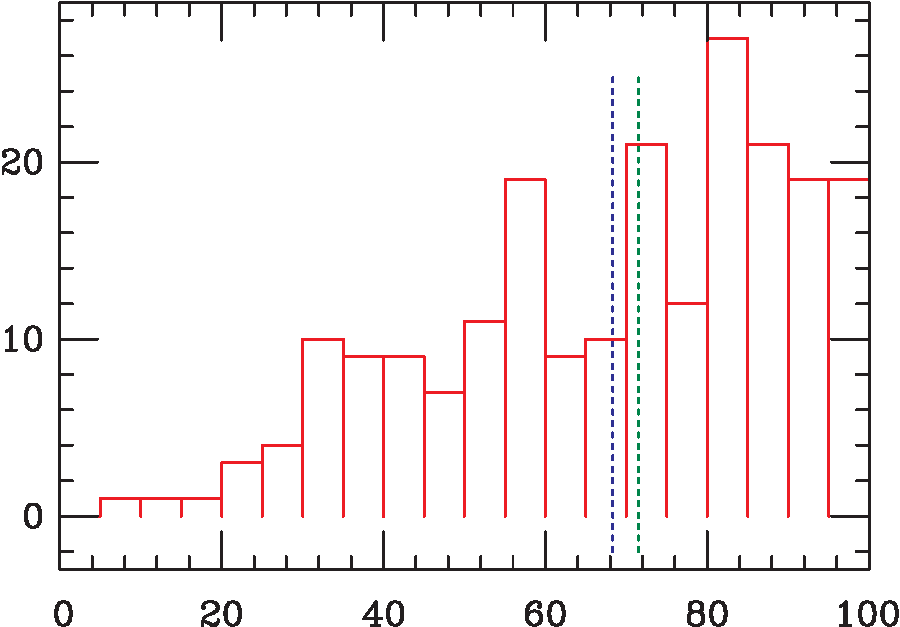
\includegraphics[width=0.6\textwidth]{../../grades/grades-crop.pdf}}
 \pause
 \centerline{Your average was 71\%}
   \pause
   \centerline{This exam was harder than earlier ones}
   \pause
   \centerline{The historical average was 60\%}
     \pause
     \centerline{Historically classes have had an extra week of prep!}
     \pause

     \bigskip
   
     \centerline{\color{Blue}I am very proud of you all!}
 
}

\frame{\frametitle{\textbf{Ask a Physicist: Water wheels and power stations}}
}

  \frame{\frametitle{\textbf{Forces so far:}}
    \BI
\Large  \item{Gravity}
  \BI
\normalsize\item{Every object near Earth feels a force with magnitude $mg$ directed downward. No exceptions!}

  \bigskip
  
  \EI
\Large \item{Normal forces}
\BI
\normalsize\item{Always directed normal (perpendicular) to a surface}
\item{Magnitude is as large as it needs to be to stop objects from ``crossing'' ($a_\perp = 0$)}
\item{Newton's third law: if A pushes on B, B pushes back on A (the book problem)}
  \EI

\bigskip

\Large\item{Tension}
\BI
\normalsize\item{The force transmitted through a rope from one thing to another}
\item{Same on both sides of the rope (Newton's 3rd...)}
  \EI
  \EI
  }

  \frame{\frametitle{\textbf{Force diagrams}}
    \large
    \BI
  \item{Accounting devices for your use, to keep straight forces for $\vec F = m \vec a$}
\item{Some guidelines:}
  \BI
\item{Draw a {\color{Red}separate diagram} for each object (book problem again!)}
\item{Each force gets a separate arrow}
\item{Draw them {\color{Red}big enough} that you can draw ``component-triangles''}
\item{``Net force'', velocity, acceleration not forces; only physical agents are}
  \EI
  \EI
  \small
  \centerline{(Examples on document camera)}

  }

  \frame{\frametitle{\textbf{Forces in 2D (and 3D)}}
    \large
    \centerline{Force is a vector; handle it like any other}

\bigskip
\bigskip
\bigskip

    \centerline{One copy of Newton's second law in each direction (per object)}

    \bigskip

    \centerline{ \Large $\vec F = m \vec a \rightarrow {{F_x = m a_x} \choose {F_y = m a_y}}$}

  \bigskip

  \pause


  \bigskip
  \bigskip
  \bigskip


  \normalsize
  
  
  Important: When dealing with inclines, choose your axes to align with the incline! ($F_N$ is easy that way)



}

\frame{\frametitle{\textbf{A problem-solving recipe (remember this!)}}
  \large
\BI
\item{{\color{Red}Accounting:} Draw force diagrams for every object}
  \BI
\item{Work out components (trigonometry) of vectors in funny directions -- no need for numbers}
  \EI
  \pause
\item{{\color{Red}Physics:} Write down $\sum F = ma$ in each dimension, for each object}
  \pause
\item{{\color{Red}Math:} Put in the stuff you know, solve for the stuff you don't}
  \pause
\item{{\color{Red}Kinematics:} Connect acceleration to motion}
  \EI
\pause

\bigskip
\bigskip

\centerline{It really is this easy; I promise!}
\pause
\centerline{``Ask physics the question, don't tell it the answer''}

}



  \frame{\frametitle{\textbf{Sample questions}}
    \Large

    A stone hangs from the roof of a car by a string; the car accelerates forward at 3 $\rm m/\rm s^2$.

    \BI
  \item{What happens to the string?}
    \pause
  \item{What angle does the string make with the vertical?}
    \pause
  \item{What is the tension in the string?}
    \EI
  }

  \frame{\frametitle{\textbf{Sample questions}}
    \Large

    A cart slides down a frictionless track elevated at angle $\theta$; what is its acceleration?

    \BI
  \item{What happens to the string?}
    \pause
  \item{What angle does the string make with the vertical?}
    \pause
  \item{What is the tension in the string?}
    \EI
  } 

  \frame{\frametitle{\textbf{Sample questions}}
    \Large

    Two masses of 20 and 40 kg hang from a massless pulley on either side. How do they move?
  } 

  \frame{\frametitle{\textbf{Sample questions}}
    \Large

    Two masses of $m_1$ and $m_2$ kg hang from a massless pulley on either side. How do they move?
  } 


  \end{document}

